\documentclass[]{ctexbook}
\usepackage{lmodern}
\usepackage{amssymb,amsmath}
\usepackage{ifxetex,ifluatex}
\usepackage{fixltx2e} % provides \textsubscript
\ifnum 0\ifxetex 1\fi\ifluatex 1\fi=0 % if pdftex
  \usepackage[T1]{fontenc}
  \usepackage[utf8]{inputenc}
\else % if luatex or xelatex
  \ifxetex
    \usepackage{xltxtra,xunicode}
  \else
    \usepackage{fontspec}
  \fi
  \defaultfontfeatures{Ligatures=TeX,Scale=MatchLowercase}
\fi
% use upquote if available, for straight quotes in verbatim environments
\IfFileExists{upquote.sty}{\usepackage{upquote}}{}
% use microtype if available
\IfFileExists{microtype.sty}{%
\usepackage{microtype}
\UseMicrotypeSet[protrusion]{basicmath} % disable protrusion for tt fonts
}{}
\usepackage[b5paper,tmargin=2.5cm,bmargin=2.5cm,lmargin=3.5cm,rmargin=2.5cm]{geometry}
\usepackage[unicode=true]{hyperref}
\PassOptionsToPackage{usenames,dvipsnames}{color} % color is loaded by hyperref
\hypersetup{
            pdftitle={R中的统计模拟},
            pdfauthor={wang},
            colorlinks=true,
            linkcolor=Maroon,
            citecolor=Blue,
            urlcolor=Blue,
            breaklinks=true}
\urlstyle{same}  % don't use monospace font for urls
\usepackage{natbib}
\bibliographystyle{apalike}
\usepackage{color}
\usepackage{fancyvrb}
\newcommand{\VerbBar}{|}
\newcommand{\VERB}{\Verb[commandchars=\\\{\}]}
\DefineVerbatimEnvironment{Highlighting}{Verbatim}{commandchars=\\\{\}}
% Add ',fontsize=\small' for more characters per line
\usepackage{framed}
\definecolor{shadecolor}{RGB}{248,248,248}
\newenvironment{Shaded}{\begin{snugshade}}{\end{snugshade}}
\newcommand{\AlertTok}[1]{\textcolor[rgb]{0.94,0.16,0.16}{#1}}
\newcommand{\AnnotationTok}[1]{\textcolor[rgb]{0.56,0.35,0.01}{\textbf{\textit{#1}}}}
\newcommand{\AttributeTok}[1]{\textcolor[rgb]{0.77,0.63,0.00}{#1}}
\newcommand{\BaseNTok}[1]{\textcolor[rgb]{0.00,0.00,0.81}{#1}}
\newcommand{\BuiltInTok}[1]{#1}
\newcommand{\CharTok}[1]{\textcolor[rgb]{0.31,0.60,0.02}{#1}}
\newcommand{\CommentTok}[1]{\textcolor[rgb]{0.56,0.35,0.01}{\textit{#1}}}
\newcommand{\CommentVarTok}[1]{\textcolor[rgb]{0.56,0.35,0.01}{\textbf{\textit{#1}}}}
\newcommand{\ConstantTok}[1]{\textcolor[rgb]{0.00,0.00,0.00}{#1}}
\newcommand{\ControlFlowTok}[1]{\textcolor[rgb]{0.13,0.29,0.53}{\textbf{#1}}}
\newcommand{\DataTypeTok}[1]{\textcolor[rgb]{0.13,0.29,0.53}{#1}}
\newcommand{\DecValTok}[1]{\textcolor[rgb]{0.00,0.00,0.81}{#1}}
\newcommand{\DocumentationTok}[1]{\textcolor[rgb]{0.56,0.35,0.01}{\textbf{\textit{#1}}}}
\newcommand{\ErrorTok}[1]{\textcolor[rgb]{0.64,0.00,0.00}{\textbf{#1}}}
\newcommand{\ExtensionTok}[1]{#1}
\newcommand{\FloatTok}[1]{\textcolor[rgb]{0.00,0.00,0.81}{#1}}
\newcommand{\FunctionTok}[1]{\textcolor[rgb]{0.00,0.00,0.00}{#1}}
\newcommand{\ImportTok}[1]{#1}
\newcommand{\InformationTok}[1]{\textcolor[rgb]{0.56,0.35,0.01}{\textbf{\textit{#1}}}}
\newcommand{\KeywordTok}[1]{\textcolor[rgb]{0.13,0.29,0.53}{\textbf{#1}}}
\newcommand{\NormalTok}[1]{#1}
\newcommand{\OperatorTok}[1]{\textcolor[rgb]{0.81,0.36,0.00}{\textbf{#1}}}
\newcommand{\OtherTok}[1]{\textcolor[rgb]{0.56,0.35,0.01}{#1}}
\newcommand{\PreprocessorTok}[1]{\textcolor[rgb]{0.56,0.35,0.01}{\textit{#1}}}
\newcommand{\RegionMarkerTok}[1]{#1}
\newcommand{\SpecialCharTok}[1]{\textcolor[rgb]{0.00,0.00,0.00}{#1}}
\newcommand{\SpecialStringTok}[1]{\textcolor[rgb]{0.31,0.60,0.02}{#1}}
\newcommand{\StringTok}[1]{\textcolor[rgb]{0.31,0.60,0.02}{#1}}
\newcommand{\VariableTok}[1]{\textcolor[rgb]{0.00,0.00,0.00}{#1}}
\newcommand{\VerbatimStringTok}[1]{\textcolor[rgb]{0.31,0.60,0.02}{#1}}
\newcommand{\WarningTok}[1]{\textcolor[rgb]{0.56,0.35,0.01}{\textbf{\textit{#1}}}}
\usepackage{longtable,booktabs}
% Fix footnotes in tables (requires footnote package)
\IfFileExists{footnote.sty}{\usepackage{footnote}\makesavenoteenv{long table}}{}
\usepackage{graphicx,grffile}
\makeatletter
\def\maxwidth{\ifdim\Gin@nat@width>\linewidth\linewidth\else\Gin@nat@width\fi}
\def\maxheight{\ifdim\Gin@nat@height>\textheight\textheight\else\Gin@nat@height\fi}
\makeatother
% Scale images if necessary, so that they will not overflow the page
% margins by default, and it is still possible to overwrite the defaults
% using explicit options in \includegraphics[width, height, ...]{}
\setkeys{Gin}{width=\maxwidth,height=\maxheight,keepaspectratio}
\IfFileExists{parskip.sty}{%
\usepackage{parskip}
}{% else
\setlength{\parindent}{0pt}
\setlength{\parskip}{6pt plus 2pt minus 1pt}
}
\setlength{\emergencystretch}{3em}  % prevent overfull lines
\providecommand{\tightlist}{%
  \setlength{\itemsep}{0pt}\setlength{\parskip}{0pt}}
\setcounter{secnumdepth}{5}
% Redefines (sub)paragraphs to behave more like sections
\ifx\paragraph\undefined\else
\let\oldparagraph\paragraph
\renewcommand{\paragraph}[1]{\oldparagraph{#1}\mbox{}}
\fi
\ifx\subparagraph\undefined\else
\let\oldsubparagraph\subparagraph
\renewcommand{\subparagraph}[1]{\oldsubparagraph{#1}\mbox{}}
\fi

% set default figure placement to htbp
\makeatletter
\def\fps@figure{htbp}
\makeatother

\usepackage{booktabs}
\usepackage{longtable}

\usepackage{framed,color}
\definecolor{shadecolor}{RGB}{248,248,248}

\renewcommand{\textfraction}{0.05}
\renewcommand{\topfraction}{0.8}
\renewcommand{\bottomfraction}{0.8}
\renewcommand{\floatpagefraction}{0.75}

\let\oldhref\href
\renewcommand{\href}[2]{#2\footnote{\url{#1}}}

\makeatletter
\newenvironment{kframe}{%
\medskip{}
\setlength{\fboxsep}{.8em}
 \def\at@end@of@kframe{}%
 \ifinner\ifhmode%
  \def\at@end@of@kframe{\end{minipage}}%
  \begin{minipage}{\columnwidth}%
 \fi\fi%
 \def\FrameCommand##1{\hskip\@totalleftmargin \hskip-\fboxsep
 \colorbox{shadecolor}{##1}\hskip-\fboxsep
     % There is no \\@totalrightmargin, so:
     \hskip-\linewidth \hskip-\@totalleftmargin \hskip\columnwidth}%
 \MakeFramed {\advance\hsize-\width
   \@totalleftmargin\z@ \linewidth\hsize
   \@setminipage}}%
 {\par\unskip\endMakeFramed%
 \at@end@of@kframe}
\makeatother

\makeatletter
\@ifundefined{Shaded}{
}{\renewenvironment{Shaded}{\begin{kframe}}{\end{kframe}}}
\@ifpackageloaded{fancyvrb}{%
  % https://github.com/CTeX-org/ctex-kit/issues/331
  \RecustomVerbatimEnvironment{Highlighting}{Verbatim}{commandchars=\\\{\},formatcom=\xeCJKVerbAddon}%
}{}
\makeatother

\usepackage{makeidx}
\makeindex

\urlstyle{tt}

\usepackage{amsthm}
\makeatletter
\def\thm@space@setup{%
  \thm@preskip=8pt plus 2pt minus 4pt
  \thm@postskip=\thm@preskip
}
\makeatother

\frontmatter

\title{R中的统计模拟}
\author{wang}
\date{2019-07-27}

\begin{document}
\maketitle


\thispagestyle{empty}

\begin{center}
献给……

呃,爱谁谁吧
\end{center}

\setlength{\abovedisplayskip}{-5pt}
\setlength{\abovedisplayshortskip}{-5pt}

{
\setcounter{tocdepth}{2}
\tableofcontents
}
\listoftables
\listoffigures
\hypertarget{section}{%
\chapter*{前言}\label{section}}


关于R的基础语法,可以在网上或者书籍中学习.

\href{https://github.com/yanping/r-spring-camp/blob/master/1-introduction.md}{Github}

\href{https://www.w3cschool.cn/r/r_overview.html}{W3Cschool}

这里只是总结一些统计模拟中遇到的问题,以及实用的技巧.

\hypertarget{section-1}{%
\section*{致谢}\label{section-1}}


这个页面的建立基于 \textbf{knitr}\index{knitr} \citep{xie2015}和 \textbf{bookdown}\index{bookdown} \citep{R-bookdown}。以下是我的 R 进程信息:

\begin{Shaded}
\begin{Highlighting}[]
\KeywordTok{sessionInfo}\NormalTok{()}
\end{Highlighting}
\end{Shaded}

\begin{verbatim}
## R version 3.6.0 (2019-04-26)
## Platform: x86_64-apple-darwin15.6.0 (64-bit)
## Running under: macOS Mojave 10.14.6
## 
## Matrix products: default
## BLAS:   /Library/Frameworks/R.framework/Versions/3.6/Resources/lib/libRblas.0.dylib
## LAPACK: /Library/Frameworks/R.framework/Versions/3.6/Resources/lib/libRlapack.dylib
## 
## locale:
## [1] en_US.UTF-8/en_US.UTF-8/en_US.UTF-8/C/en_US.UTF-8/en_US.UTF-8
## 
## attached base packages:
## [1] stats     graphics  grDevices utils     datasets 
## [6] methods   base     
## 
## loaded via a namespace (and not attached):
##  [1] Rcpp_1.0.1         plyr_1.8.4        
##  [3] pillar_1.4.1       compiler_3.6.0    
##  [5] RColorBrewer_1.1-2 influenceR_0.1.0  
##  [7] viridis_0.5.1      tools_3.6.0       
##  [9] zeallot_0.1.0      digest_0.6.19     
## [11] jsonlite_1.6       viridisLite_0.3.0 
## [13] gtable_0.3.0       evaluate_0.14     
## [15] tibble_2.1.3       rgexf_0.15.3      
## [17] pkgconfig_2.0.2    rlang_0.4.0       
## [19] igraph_1.2.4.1     rstudioapi_0.10   
## [21] yaml_2.2.0         xfun_0.7          
## [23] gridExtra_2.3      downloader_0.4    
## [25] DiagrammeR_1.0.1   dplyr_0.8.1       
## [27] stringr_1.4.0      knitr_1.23        
## [29] htmlwidgets_1.3    vctrs_0.2.0       
## [31] hms_0.5.0          grid_3.6.0        
## [33] tidyselect_0.2.5   glue_1.3.1        
## [35] R6_2.4.0           Rook_1.1-1        
## [37] XML_3.98-1.20      rmarkdown_1.13    
## [39] bookdown_0.11      ggplot2_3.1.1     
## [41] tidyr_0.8.3        purrr_0.3.2       
## [43] readr_1.3.1        magrittr_1.5      
## [45] scales_1.0.0       backports_1.1.4   
## [47] htmltools_0.3.6    assertthat_0.2.1  
## [49] colorspace_1.4-1   brew_1.0-6        
## [51] stringi_1.4.3      visNetwork_2.0.7  
## [53] lazyeval_0.2.2     munsell_0.5.0     
## [55] crayon_1.3.4
\end{verbatim}

\hypertarget{author}{%
\chapter*{作者简介}\label{author}}


统计学学生.

主要用R和tex.

\mainmatter

\hypertarget{section-2}{%
\chapter{常用函数及常见错误}\label{section-2}}

\hypertarget{section-3}{%
\section{产生数据}\label{section-3}}

在进行模拟时, 我们经常会需要生成数据. 这里以正态分布为例, 说明如 何产生数据. 在 R 中, 每种分布都会有以下 4 个函数:

\begin{itemize}
\tightlist
\item
  概率密度函数: dnorm(x, mean = 0, sd = 1, log = FALSE)
\item
  累计分布函数: pnorm(q, mean = 0, sd = 1, lower.tail = TRUE, log.p = FALSE)
\item
  分位数函数: qnorm(p, mean = 0, sd = 1, lower.tail = TRUE, log.p = FALSE)
\item
  随机数产生: rnorm(n, mean = 0, sd = 1):
\end{itemize}

其中前 3 个函数都支持向量输入, 即计算一组取值的概率密度、累计分布、 分位数. 最后一个函数常用来生成数据,n 即产生数据的个数. 如果需要生成 多维正态分布, 需要调用 MASS 包中的
*mvrnorm(n = 1, mu, Sigma, tol = 1e-6, empirical = FALSE, EISPACK = FALSE),
其中 Sigma 是指定的协方差矩阵.

\hypertarget{section-4}{%
\section{定义运算符}\label{section-4}}

空间模型 (SAR) 中, 会出现对角块矩阵 \[ \mathbf{W}=\left(\begin{array}{cccc}{\mathbf{M}} & {} & {} & {} \\ {} & {\mathbf{M}} & {} & {} \\ {} & {} & {\ddots} & {} \\ {} & {} & {} & {\mathbf{M}}\end{array}\right) \]

M 作为权重矩阵, 这种形式的矩阵可以利用克罗内克积 (Kronecker product, 符号为\(\otimes\)) 在 R 中很方便的产生,命令是\%x\%.
可以写成\[\mathbf{W} = \mathbf{I} \otimes \mathbf{M}.\]

\begin{Shaded}
\begin{Highlighting}[]
\KeywordTok{diag}\NormalTok{(}\DecValTok{3}\NormalTok{)}\OperatorTok\KeywordTok{matrix}\NormalTok{(}\DecValTok{1}\OperatorTok{:}\DecValTok{6}\NormalTok{,}\DecValTok{2}\NormalTok{,}\DecValTok{3}\NormalTok{)}
\end{Highlighting}
\end{Shaded}

\begin{verbatim}
##      [,1] [,2] [,3] [,4] [,5] [,6] [,7] [,8] [,9]
## [1,]    1    3    5    0    0    0    0    0    0
## [2,]    2    4    6    0    0    0    0    0    0
## [3,]    0    0    0    1    3    5    0    0    0
## [4,]    0    0    0    2    4    6    0    0    0
## [5,]    0    0    0    0    0    0    1    3    5
## [6,]    0    0    0    0    0    0    2    4    6
\end{verbatim}

这是借助自定义运算符实现的.自定义运算符是一种特殊的函数,当参数只有两个变量时,可以进行定义.用法如下:

\begin{Shaded}
\begin{Highlighting}[]
\StringTok{'%myop%'}\NormalTok{<-}\ControlFlowTok{function}\NormalTok{(a,b)\{a}\OperatorTok{^}\NormalTok{b}\OperatorTok{+}\NormalTok{b}\OperatorTok{^}\NormalTok{a\}}
\DecValTok{2}\OperatorTok\DecValTok{3}
\end{Highlighting}
\end{Shaded}

\begin{verbatim}
## [1] 17
\end{verbatim}

利用自定义运算符,可以实现很方便的功能.R中矩阵乘法(\%*\%)、Kronecker乘积(\%x\%)都是这样实现的.另外还有整除(\%/\%)和取余(\%\%)

\begin{Shaded}
\begin{Highlighting}[]
\DecValTok{9}\OperatorTok\DecValTok{4}
\end{Highlighting}
\end{Shaded}

\begin{verbatim}
## [1] 2
\end{verbatim}

\begin{Shaded}
\begin{Highlighting}[]
\DecValTok{13}\OperatorTok\DecValTok{3}
\end{Highlighting}
\end{Shaded}

\begin{verbatim}
## [1] 1
\end{verbatim}

\hypertarget{section-5}{%
\section{自动纠错}\label{section-5}}

当我们输入的命令不规范时,R会自动纠正,以保证程序正常运行.

比如看下面的例子:

\begin{Shaded}
\begin{Highlighting}[]
\DecValTok{1}\OperatorTok{:}\DecValTok{4} \OperatorTok{-}\StringTok{ }\DecValTok{1}\OperatorTok{:}\DecValTok{2}
\end{Highlighting}
\end{Shaded}

\begin{verbatim}
## [1] 0 0 2 2
\end{verbatim}

\begin{Shaded}
\begin{Highlighting}[]
\DecValTok{1}\OperatorTok{:}\DecValTok{5-1}\OperatorTok{:}\DecValTok{2}
\end{Highlighting}
\end{Shaded}

\begin{verbatim}
## Warning in 1:5 - 1:2: longer object length is not a
## multiple of shorter object length
\end{verbatim}

\begin{verbatim}
## [1] 0 0 2 2 4
\end{verbatim}

当运算的向量长度不一致时,R会自动重复短的向量,使之长度与另外的向量长度相同进行运算.但是当长度是整数倍当时候,不会有任何提示.

再看下面当例子:

\begin{Shaded}
\begin{Highlighting}[]
\KeywordTok{matrix}\NormalTok{(}\DecValTok{1}\OperatorTok{:}\DecValTok{9}\NormalTok{,}\DecValTok{3}\NormalTok{,}\DecValTok{3}\NormalTok{)}\OperatorTok{*}\NormalTok{(}\DecValTok{1}\OperatorTok{:}\DecValTok{3}\NormalTok{)}
\end{Highlighting}
\end{Shaded}

\begin{verbatim}
##      [,1] [,2] [,3]
## [1,]    1    4    7
## [2,]    4   10   16
## [3,]    9   18   27
\end{verbatim}

本来想计算矩阵与向量的乘积,但是错误使用了*,
未使用矩阵乘法\%*\%,R也可以计算返回一个矩阵,不会有warning.

当条件为向量是,只会判断第一个值:

\begin{Shaded}
\begin{Highlighting}[]
\ControlFlowTok{if}\NormalTok{( }\DecValTok{1} \OperatorTok{<=}\StringTok{ }\DecValTok{1}\OperatorTok{:}\DecValTok{3}\NormalTok{) }\KeywordTok{print}\NormalTok{(}\StringTok{"真"}\NormalTok{)  }\ControlFlowTok{else} \KeywordTok{print}\NormalTok{(}\StringTok{"假"}\NormalTok{)}
\end{Highlighting}
\end{Shaded}

\begin{verbatim}
## Warning in if (1 <= 1:3) print("真") else print("假"):
## the condition has length > 1 and only the first element
## will be used
\end{verbatim}

\begin{verbatim}
## [1] "真"
\end{verbatim}

如果条件为向量,应该使用all或者any函数:

\begin{Shaded}
\begin{Highlighting}[]
\KeywordTok{all}\NormalTok{(}\DecValTok{1} \OperatorTok{<=}\StringTok{ }\DecValTok{1}\OperatorTok{:}\DecValTok{3}\NormalTok{)}
\end{Highlighting}
\end{Shaded}

\begin{verbatim}
## [1] TRUE
\end{verbatim}

\begin{Shaded}
\begin{Highlighting}[]
\KeywordTok{all}\NormalTok{(}\DecValTok{2} \OperatorTok{<=}\StringTok{ }\DecValTok{1}\OperatorTok{:}\DecValTok{3}\NormalTok{)}
\end{Highlighting}
\end{Shaded}

\begin{verbatim}
## [1] FALSE
\end{verbatim}

所有都真的时候返回TRUE.

\begin{Shaded}
\begin{Highlighting}[]
\KeywordTok{any}\NormalTok{(}\DecValTok{4} \OperatorTok{<=}\StringTok{ }\DecValTok{1}\OperatorTok{:}\DecValTok{3}\NormalTok{)}
\end{Highlighting}
\end{Shaded}

\begin{verbatim}
## [1] FALSE
\end{verbatim}

\begin{Shaded}
\begin{Highlighting}[]
\KeywordTok{any}\NormalTok{(}\DecValTok{2} \OperatorTok{<=}\StringTok{ }\DecValTok{1}\OperatorTok{:}\DecValTok{3}\NormalTok{)}
\end{Highlighting}
\end{Shaded}

\begin{verbatim}
## [1] TRUE
\end{verbatim}

只要有一个为真就返回TRUE.

\hypertarget{predict}{%
\section{predict函数}\label{predict}}

当我们拟合好一个模型时,下一步要做的就是评价模型好坏或者对新数据预测.这都需要将新的输入值带入模型中计算,得到预测值.区别只是有没有真值对比.对于简单模型,我们当然可以直接提取系数,自己计算预测值,但是当模型复杂时(比如时间序列模型),就不太容易操作.

R借助泛型函数\footnote{泛型函数简单讲就是根据输入数据类型,会自动匹配对应的计算方法.比如plot函数,传入1维向量、矩阵,程序都会正确画图.泛型函数的声明需要使用``.'',在自己编写函数时,最好不要用``.''.},编写模型都会提供summary、predict、plot等函数方便调用.但是在学习过程中发现经常会不小心错误使用,特此单独说明一下.下面以线性模型为例,先看正确的使用方法:

\begin{Shaded}
\begin{Highlighting}[]
\NormalTok{n=}\DecValTok{100}\NormalTok{;p=}\DecValTok{3}\NormalTok{;beta=}\KeywordTok{c}\NormalTok{(}\DecValTok{1}\NormalTok{,}\DecValTok{2}\NormalTok{,}\DecValTok{3}\NormalTok{);}
\NormalTok{X =}\StringTok{ }\KeywordTok{matrix}\NormalTok{(}\KeywordTok{rnorm}\NormalTok{(n}\OperatorTok{*}\NormalTok{p),n,p)}
\NormalTok{Y =}\StringTok{ }\NormalTok{X}\OperatorTok\NormalTok{beta }\OperatorTok{+}\StringTok{ }\KeywordTok{rnorm}\NormalTok{(n)}
\NormalTok{trainlist =}\StringTok{ }\KeywordTok{sample}\NormalTok{(}\DecValTok{1}\OperatorTok{:}\NormalTok{n,}\DecValTok{70}\NormalTok{)}
\NormalTok{regData =}\StringTok{ }\KeywordTok{data.frame}\NormalTok{(Y,X)}
\NormalTok{fitmodel =}\StringTok{ }\KeywordTok{lm}\NormalTok{(Y}\OperatorTok{~}\NormalTok{.,}\DataTypeTok{data=}\NormalTok{regData[trainlist,])}
\NormalTok{pe =}\StringTok{ }\KeywordTok{predict}\NormalTok{(fitmodel,}\DataTypeTok{newdata=}\NormalTok{regData[}\OperatorTok{-}\NormalTok{trainlist,])}
\KeywordTok{sum}\NormalTok{((pe}\OperatorTok{-}\NormalTok{regData[}\OperatorTok{-}\NormalTok{trainlist,}\DecValTok{1}\NormalTok{])}\OperatorTok{^}\DecValTok{2}\NormalTok{)}\OperatorTok{/}\KeywordTok{length}\NormalTok{(pe)}
\end{Highlighting}
\end{Shaded}

\begin{verbatim}
## [1] 0.6623
\end{verbatim}

关键点:

\emph{所有数据存在一个数据框中
}通过下标控制训练集和测试集的数据

错误程序1:

\begin{Shaded}
\begin{Highlighting}[]
\NormalTok{n=}\DecValTok{100}\NormalTok{;p=}\DecValTok{3}\NormalTok{;beta=}\KeywordTok{c}\NormalTok{(}\DecValTok{1}\NormalTok{,}\DecValTok{2}\NormalTok{,}\DecValTok{3}\NormalTok{);}
\NormalTok{X =}\StringTok{ }\KeywordTok{matrix}\NormalTok{(}\KeywordTok{rnorm}\NormalTok{(n}\OperatorTok{*}\NormalTok{p),n,p)}
\NormalTok{Y =}\StringTok{ }\NormalTok{X}\OperatorTok\NormalTok{beta }\OperatorTok{+}\StringTok{ }\KeywordTok{rnorm}\NormalTok{(n)}
\NormalTok{fitmodel =}\StringTok{ }\KeywordTok{lm}\NormalTok{(Y}\OperatorTok{~}\NormalTok{X)}
\NormalTok{X2 =}\StringTok{ }\KeywordTok{matrix}\NormalTok{(}\KeywordTok{rnorm}\NormalTok{(n}\OperatorTok{*}\NormalTok{p),n,p)}
\NormalTok{Y2 =}\StringTok{ }\NormalTok{X2}\OperatorTok\NormalTok{beta }\OperatorTok{+}\StringTok{ }\KeywordTok{rnorm}\NormalTok{(n)}
\CommentTok{#predict(fitmodel,newdata = X2)数据格式错误,不能执行}
\NormalTok{pe =}\StringTok{ }\KeywordTok{predict}\NormalTok{(fitmodel,}\DataTypeTok{newdata =} \KeywordTok{data.frame}\NormalTok{(X2))}
\KeywordTok{sum}\NormalTok{((pe}\OperatorTok{-}\NormalTok{Y2)}\OperatorTok{^}\DecValTok{2}\NormalTok{)}\OperatorTok{/}\KeywordTok{length}\NormalTok{(Y2)}
\end{Highlighting}
\end{Shaded}

\begin{verbatim}
## [1] 26.06
\end{verbatim}

这个程序能明显看出问题,误差不应该这么大,但是程序没有任何warning.

错误程序2:

\begin{Shaded}
\begin{Highlighting}[]
\NormalTok{n=}\DecValTok{100}\NormalTok{;p=}\DecValTok{3}\NormalTok{;beta=}\KeywordTok{c}\NormalTok{(}\DecValTok{1}\NormalTok{,}\DecValTok{2}\NormalTok{,}\DecValTok{3}\NormalTok{);}
\NormalTok{X =}\StringTok{ }\KeywordTok{matrix}\NormalTok{(}\KeywordTok{rnorm}\NormalTok{(n}\OperatorTok{*}\NormalTok{p),n,p)}
\NormalTok{Y =}\StringTok{ }\NormalTok{X}\OperatorTok\NormalTok{beta }\OperatorTok{+}\StringTok{ }\KeywordTok{rnorm}\NormalTok{(n)}
\NormalTok{fitmodel =}\StringTok{ }\KeywordTok{lm}\NormalTok{(Y}\OperatorTok{~}\NormalTok{X)}
\NormalTok{X2 =}\StringTok{ }\KeywordTok{matrix}\NormalTok{(}\KeywordTok{rnorm}\NormalTok{(}\FloatTok{0.2}\OperatorTok{*}\NormalTok{n}\OperatorTok{*}\NormalTok{p),}\FloatTok{0.2}\OperatorTok{*}\NormalTok{n,p)}
\NormalTok{Y2 =}\StringTok{ }\NormalTok{X2}\OperatorTok\NormalTok{beta }\OperatorTok{+}\StringTok{ }\KeywordTok{rnorm}\NormalTok{(}\FloatTok{0.2}\OperatorTok{*}\NormalTok{n)}
\NormalTok{pe =}\StringTok{ }\KeywordTok{predict}\NormalTok{(fitmodel,}\DataTypeTok{newdata =} \KeywordTok{data.frame}\NormalTok{(X2))}
\end{Highlighting}
\end{Shaded}

\begin{verbatim}
## Warning: 'newdata' had 20 rows but variables found have
## 100 rows
\end{verbatim}

\begin{Shaded}
\begin{Highlighting}[]
\KeywordTok{length}\NormalTok{(pe)}
\end{Highlighting}
\end{Shaded}

\begin{verbatim}
## [1] 100
\end{verbatim}

修改测试数据的条数,使之与训练集数据量不同,可以发现warning.提示我们数据行数不一样.并且我们测试集合X2是20行,但是预测值pe返回的是100个值.问题在于predict函数使用不正确.

我们用all指令查看:

\begin{Shaded}
\begin{Highlighting}[]
\KeywordTok{all}\NormalTok{(}\KeywordTok{predict}\NormalTok{(fitmodel)}\OperatorTok{==}\KeywordTok{predict}\NormalTok{(fitmodel,}\DataTypeTok{newdata =} \KeywordTok{data.frame}\NormalTok{(X2)))}
\end{Highlighting}
\end{Shaded}

\begin{verbatim}
## Warning: 'newdata' had 20 rows but variables found have
## 100 rows
\end{verbatim}

\begin{verbatim}
## [1] TRUE
\end{verbatim}

查看函数说明

\begin{Shaded}
\begin{Highlighting}[]
\NormalTok{?predict.lm}
\end{Highlighting}
\end{Shaded}

\begin{longtable}[]{@{}ll@{}}
\toprule
\begin{minipage}[b]{0.13\columnwidth}\raggedright
参数\strut
\end{minipage} & \begin{minipage}[b]{0.81\columnwidth}\raggedright
说明\strut
\end{minipage}\tabularnewline
\midrule
\endhead
\begin{minipage}[t]{0.13\columnwidth}\raggedright
object\strut
\end{minipage} & \begin{minipage}[t]{0.81\columnwidth}\raggedright
Object of class inheriting from ``lm''\strut
\end{minipage}\tabularnewline
\begin{minipage}[t]{0.13\columnwidth}\raggedright
newdata\strut
\end{minipage} & \begin{minipage}[t]{0.81\columnwidth}\raggedright
An optional data frame in which to look for variables with which to predict. If omitted, the fitted values are used.\strut
\end{minipage}\tabularnewline
\bottomrule
\end{longtable}

newdata不是必要的参数,当缺失时候会使用拟合模型的数据.

通过以上例子,想说明当程序的结果和预期不一致时.当然可能是我们的方法不对,但是也有可能是调用函数的方式出了问题.比如线性规划求解的lp函数,默认在正半轴求解\footnote{因为任何一个实数可以分解成两个非负数的差,将搜索范围限定到正半轴,求解程序更好实现.}.

\hypertarget{section-6}{%
\section{保存结果}\label{section-6}}

\hypertarget{section-7}{%
\section{结果输出}\label{section-7}}

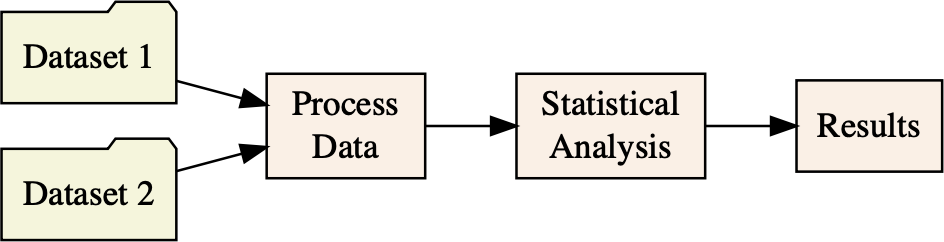
\includegraphics{bookdown_files/figure-latex/流程图-1.png}

\hypertarget{section-8}{%
\chapter{常见错误}\label{section-8}}

自动调整

\hypertarget{section-9}{%
\chapter{参数估计}\label{section-9}}

\hypertarget{m}{%
\section{M估计}\label{m}}

\hypertarget{z}{%
\section{Z估计}\label{z}}

\hypertarget{section-10}{%
\chapter{假设检验}\label{section-10}}

\hypertarget{section-11}{%
\chapter{进阶技巧}\label{section-11}}

\hypertarget{apply}{%
\section{apply函数族}\label{apply}}

\hypertarget{section-12}{%
\section{并行}\label{section-12}}

\hypertarget{rcpp}{%
\section{Rcpp}\label{rcpp}}

\cleardoublepage

\hypertarget{appendix-}{%
\appendix \addcontentsline{toc}{chapter}{\appendixname}}


\hypertarget{sound}{%
\chapter{余音绕梁}\label{sound}}

呐,到这里朕的书差不多写完了,但还有几句话要交待,所以开个附录,再啰嗦几句,各位客官稍安勿躁、扶稳坐好。

\bibliography{book.bib,packages.bib}

\backmatter
\printindex

\end{document}
